
% This LaTeX was auto-generated from MATLAB code.
% To make changes, update the MATLAB code and republish this document.

\documentclass{article}
\usepackage{graphicx}
\usepackage{color}

\sloppy
\definecolor{lightgray}{gray}{0.5}
\setlength{\parindent}{0pt}

\begin{document}

    
    
\section*{Tutorialanwendung}

\begin{par}
Zur Demonstration der AMrotorSIM-Toolbox
\end{par} \vspace{1em}

\subsection*{Contents}

\begin{itemize}
\setlength{\itemsep}{-1ex}
   \item Header
   \item Import
   \item Clean up
   \item Compute Rotor
   \item Running system analyses
   \item Running Time Simulation
\end{itemize}


\subsection*{Header}

\begin{verbatim}
% Johannes Maierhofer
% 28.03.2017,29.03.2017,30.03.2017,31.03.2017,03.04.2017,04.04.2017,05.04.2017,06.04.2017
%
%      .o.       ooo        ooooo                        .
%     .888.      `88.       .888'                      .o8
%    .8"888.      888b     d'888  oooo d8b  .ooooo.  .o888oo  .ooooo.  oooo d8b
%   .8' `888.     8 Y88. .P  888  `888""8P d88' `88b   888   d88' `88b `888""8P
%  .88ooo8888.    8  `888'   888   888     888   888   888   888   888  888
% .8'     `888.   8    Y     888   888     888   888   888 . 888   888  888
%o88o     o8888o o8o        o888o d888b    `Y8bod8P'   "888" `Y8bod8P' d888b
\end{verbatim}


\subsection*{Import}

\begin{verbatim}
%import AMrotorMONI.*
import AMrotorSIM.*
\end{verbatim}


\subsection*{Clean up}

\begin{verbatim}
close all
clear all
clc
\end{verbatim}


\subsection*{Compute Rotor}

\begin{verbatim}
Config_Sim

r=Rotorsystem(cnfg,'System');
r.show;

r.rotor.mesh()
%g=Graphs.Visu_Rotorgeometrie(r.rotor);
%g.show();

g=Graphs.Visu_Rotorsystem(r);
g.show();

r.compute_matrices();
r.compute_loads();
r.reduce_modal(10);

%r.sichern();
\end{verbatim}

        \color{lightgray} \begin{verbatim}--------------- Rotorsystem --------------
System
Testrotor vom Feinsten
Zusatzscheibe
Locker l�ssiges Lager
Straffes l�ssiges Lager
----------------------------------------------
--------------- Sensors ------------------------
Sepp
Hans
----------------------------------------------
--------------- Loads ------------------------
Geplante Unwucht
----------------------------------------------
Mesh ....
Rotor Gesamtsystem
Berechne Lagersteifigkeit
Berechne Lagersteifigkeit
\end{verbatim} \color{black}
    
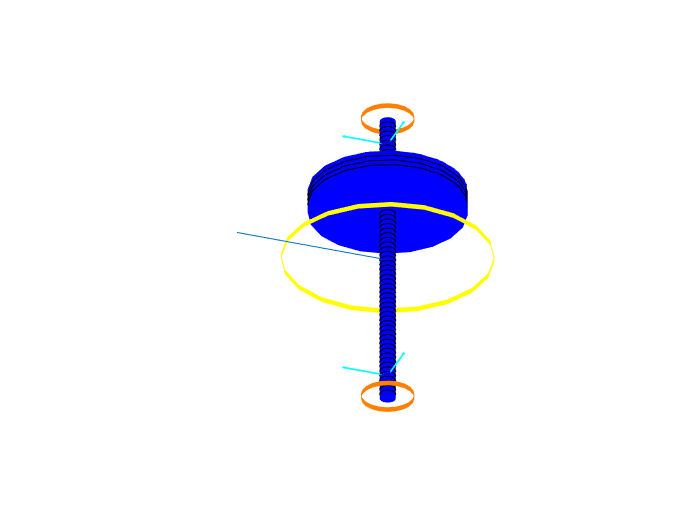
\includegraphics [width=4in]{Anwendung_01.eps}


\subsection*{Running system analyses}

\begin{verbatim}
%Modalanalyse(r).show()
\end{verbatim}


\subsection*{Running Time Simulation}

\begin{verbatim}
 St_Lsg = Experiments.Stationaere_Lsg(r,100,0:1e-3:5);
 St_Lsg.show()
 St_Lsg.compute()
%
 w = Graphs.Wegorbit(r);
 w.plot(r.sensors(1:2));
\end{verbatim}

        \color{lightgray} \begin{verbatim}Station�re L�sung
Compute.... ode15 ....
 ---   Plot Wegorbit   ---
\end{verbatim} \color{black}
    
\includegraphics [width=4in]{Anwendung_02.eps}

\includegraphics [width=4in]{Anwendung_03.eps}



\end{document}
    
